
\begin{tikzpicture}[node distance=3.4cm and 2.3cm]

% ----------------------------------------------------------
% (1) crisp 5×5 distance matrix
% ----------------------------------------------------------
\node[matrixbox] (crisp) {
  \begin{tikzpicture}[scale=0.55,baseline]
    \foreach \i in {0,...,5}{
      \draw[very thin,gray!65] (0,\i) -- (5,\i);
      \draw[very thin,gray!65] (\i,0) -- (\i,5);
    }
  \end{tikzpicture}
};
\node[below=4pt of crisp] {\scriptsize Crisp distance matrix $\mathbf{D}$};

% ----------------------------------------------------------
% (2) stack of 5 membership matrices (3×3 each)
% ----------------------------------------------------------
\foreach \name/\x/\col in {close/0/closec,midclose/1/midclosec,mid/2/midc,midfar/3/midfarc,far/4/farc}{
  \node[fuzzymatrix=\col,right=of crisp,xshift={(\x)*0.34cm-0.34cm}] (M\name){
    \begin{tikzpicture}[scale=0.29]
      \foreach \i in {0,...,3}{
        \draw[very thin,white] (0,\i) -- (3,\i);
        \draw[very thin,white] (\i,0) -- (\i,3);
      }
    \end{tikzpicture}
  };
}
\node[below=4pt of Mmid,align=center]
  {\scriptsize 5 fuzzy membership matrices\\[-1pt]\scriptsize (one per linguistic term)};

% ----------------------------------------------------------
% (3) 3×3 active-day matrix with blue shade & stair
% ----------------------------------------------------------
\node[matrixbox,right=of Mmidfar,xshift=1.1cm] (pairs) {
  \begin{tikzpicture}[scale=0.65,baseline]
    % 3×3 grid
    \foreach \i in {0,...,3}{
      \draw[very thin,gray!65] (0,\i) -- (3,\i);
      \draw[very thin,gray!65] (\i,0) -- (\i,3);
    }
    % shade cells strictly above diagonal
    \foreach \row/\col in {0/1,0/2,1/2}{
      \fill[closec!28] (\col,3-\row-1) rectangle ++(1,1);
    }
    % orange stair (border directly above diagonal) –– **top segment removed**
    \draw[midfarc,ultra thick]
      (1,3) -- (1,2) -- (2,2) -- (2,1) -- (3,1);
  \end{tikzpicture}
};
\node[below=5pt of pairs,align=center]
  {\scriptsize unique pairs (upper-triangular)\\[-1pt]\scriptsize of \emph{active-day} matrix};

% ----------------------------------------------------------
% (4) daily mass series
% ----------------------------------------------------------
\node[matrixbox,right=of pairs] (mass) {
  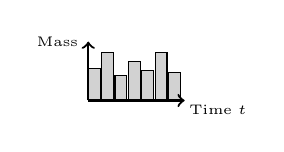
\begin{tikzpicture}[scale=0.34,baseline]
    \foreach \t/\h in {0/1.2,1/1.8,2/0.95,3/1.45,4/1.13,5/1.8,6/1.05}{
      \draw[fill=gray!35] (\t*0.50,0) rectangle ++(0.44,\h);
    }
    \draw[->,thick] (0,0) -- (3.6,0) node[below right=-2pt] {\tiny Time $t$};
    \draw[->,thick] (0,0) -- (0,2.2) node[left] {\tiny Mass};
  \end{tikzpicture}
};
\node[below=4pt of mass] {\scriptsize daily mass series $M(t)$};

% ----------------------------------------------------------
% (5) entropy scores
% ----------------------------------------------------------
\node[scalarbox,right=of mass] (entropy)
  {\Large$\displaystyle\frac{H\!\bigl(M_{\text{norm}}\bigr)}{H_{\text{unif}}}$};
\node[below=4pt of entropy,align=center]
  {\scriptsize 5 normalised entropy scores\\[-1pt]\scriptsize (one for each fuzzy term)};

% ----------------------------------------------------------
% arrows
% ----------------------------------------------------------
% Arrow 1: crisp → membership  (slightly longer, label higher)
\draw[arrow] (crisp.east) -- ++(1.0,0) -- (Mclose.west)
  node[process,above,yshift=12pt,pos=0]{apply\\linguistic\\ variable};

% Arrow 2: membership → pairs
\draw[arrow] (Mmidfar.east) -- ++(0.9,0) -- (pairs.west)
  node[process,above,yshift=12pt,pos=0.4]%
       {extract active interventions\\(submatrix)\par\textbf{for each of the 5}\\membership matrices};

% Arrow 3: pairs → mass
\draw[arrow] (pairs.east) -- (mass.west)
  node[process,above,yshift=12pt,pos=0.5]{aggregate\\per day};

% Arrow 4: mass → entropy
\draw[arrow] (mass.east) -- (entropy.west)
  node[process,above,yshift=12pt,pos=0.5]{normalise by\\total mass};

\end{tikzpicture}